% ---
% Capa
% ---
\imprimircapa
% ---

% ---
% Folha de rosto
% (o * indica que haverá a ficha bibliográfica)
% ---
\imprimirfolhaderosto*
% ---

% ---
% Inserir a ficha bibliografica
% ---
% http://ficha.bu.ufsc.br/
\begin{fichacatalografica}
	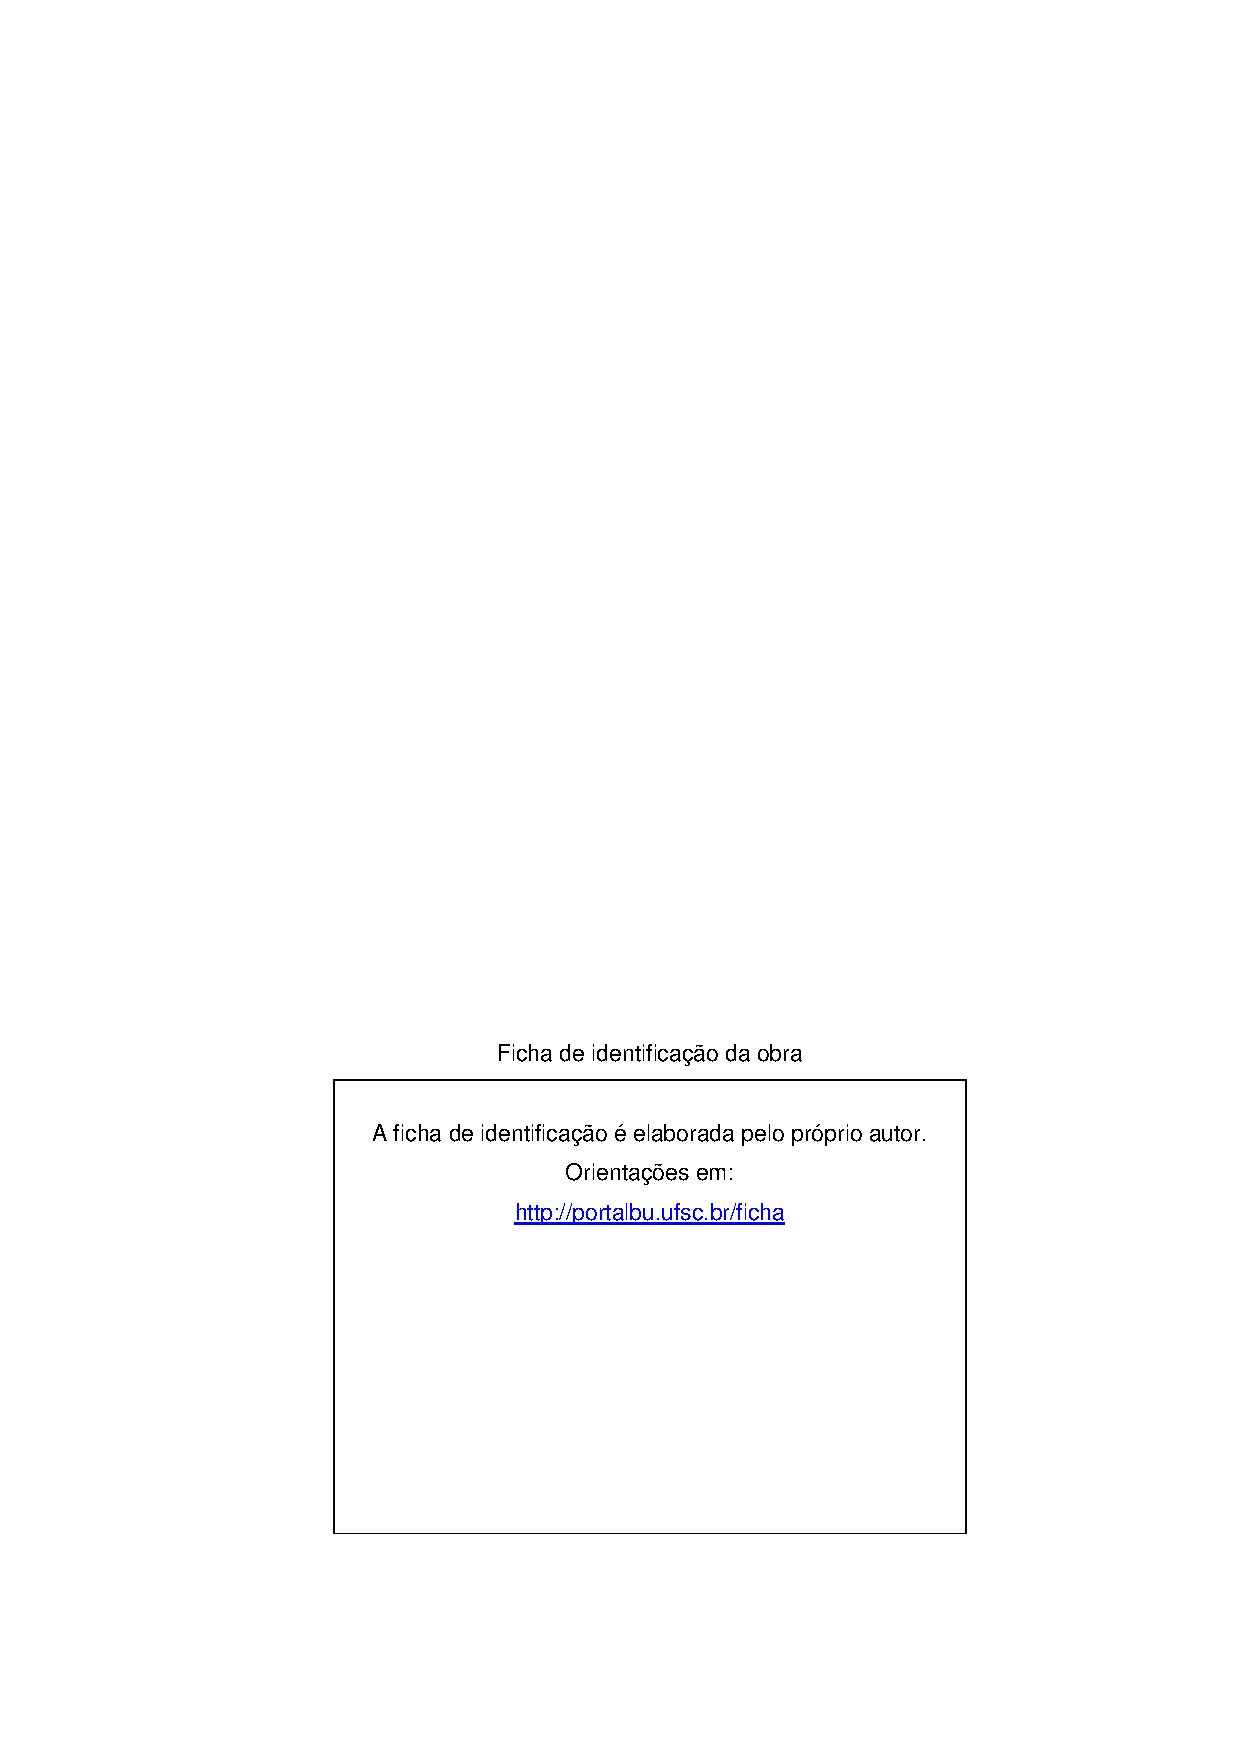
\includepdf{beforetext/Ficha_Catalografica.pdf}
\end{fichacatalografica}
% ---

% ---
% Inserir folha de aprovação
% ---
\begin{folhadeaprovacao}
	\OnehalfSpacing
	\centering
	\imprimirautor\\%
	\vspace*{10pt}		
	\textbf{\imprimirtitulo}%
	\ifnotempty{\imprimirsubtitulo}{:~\imprimirsubtitulo}\\%
	%		\vspace*{31.5pt}%3\baselineskip
	\vspace*{\baselineskip}
	
	Esta monografia foi julgada no contexto da disciplina DAS5511 (Projeto de Fim de Curso) e aprovada em sua forma final pelo \imprimircurso\\
	\vspace*{\baselineskip}
	Florianópolis, <dia(número)> de <mês> de <ano(número)>.\\
	
	%%%%%%%%%%%%%%%%%%%%%%%%%%%%%%%%%%%%%%%%%%%%%%%%%
	%IMPORTANTE: não é necessário assinaturas abaixo!
	%%%%%%%%%%%%%%%%%%%%%%%%%%%%%%%%%%%%%%%%%%%%%%%%%
	
	\vspace*{2\baselineskip}
	%\rule{0.4\textwidth}{0.4pt}\\
	Prof. Marcelo De Lellis Costa De Oliveira, Dr.\\
	Coordenador do Curso\\
	
	\vspace*{\baselineskip}
	\textbf{Banca Examinadora:} \\ \emph{[preencher somente após a defesa para a Versão Final da BU]} \\
	
	
	\vspace*{2\baselineskip}
	%\rule{0.4\textwidth}{0.4pt}\\
	Prof(a). Carlos Barros Montez, Dr.\\
	Orientador(a) \\
	UFSC/CTC/EAS\\
	
	\vspace*{2\baselineskip}
	%\rule{0.4\textwidth}{0.4pt}\\
	Matheus Fischer, Eng.\\
	Supervisor(a) \\
	Fischertec Tecnologia\\
	
	\vspace*{2\baselineskip}
	%\rule{0.4\textwidth}{0.4pt}\\
	Prof(a). xxxx, Dr(a).\\
	Avaliador(a) \\
	Instituição xxxx\\
	
	\vspace*{2\baselineskip}
	%\rule{0.4\textwidth}{0.4pt}\\
	Prof. xxxx, Dr.\\
	Presidente da Banca \\
	UFSC/CTC/EAS
\end{folhadeaprovacao}
% ---

% ---
% Dedicatória
% ---
\begin{dedicatoria}
	\vspace*{\fill}
	\noindent
	\begin{adjustwidth*}{}{5.5cm} 
		\raggedleft
		Este trabalho é dedicado aos meus amigos, colegas de classe, namorada e aos meus queridos pais.
	\end{adjustwidth*}
\end{dedicatoria}
% ---

% ---
% Agradecimentos
% ---
\begin{agradecimentos}
	Primeiramente, expresso minha gratidão à minha família, que sempre me incentivou a seguir meus sonhos acadêmicos. Agradeço particularmente à minha mãe Sandra Vicenzi e meu pai Sergio Vicenzi, pelo seu amor incondicional e pela confiança depositada em mim. Também quero mencionar minha irmã Micheli e meu cunhado Matheus, que sempre me fornecem suporte e ajuda nas horas difíceis.

	Agradeço também à minha avó Vilma e à minha tia Samara e tio Celso, que sempre me inspiraram a manter o foco e buscar excelência em tudo que faço. Por fim, quero destacar minha namorada Monike, que compartilha comigo todo o amor e paciência durante os momentos mais ansiosos da minha trajetória acadêmica. Seu apoio foi essencial para manter me motivado e garantir que todo o trabalho fosse feito com qualidade e entusiasmo.

	Agradeço ao meus colegas de classe da turma da Automação 16.2, cuja amizade e colaboração fizeram toda a diferença no desenvolvimento deste projeto. Seus comentários e sugestões foram essenciais para refinar ideias e garantir que o trabalho fosse realizado com excelência. O apoio da turma foi fonte de inspiração para manter me motivado durante os momentos mais desafiadores.

	Em seguida, quero expressar minha gratidão pelo incrível suporte recebido por meu orientador acadêmico, Carlos Montez. Sua sabedoria, paciência e expertise foram fundamentais para guiar meus passos acadêmicos, permitindo que eu avançasse com confiança no caminho da excelência na pesquisa e desenvolvimento.

	Também quero agradecer ao meu supervisor Matheus Fischer por proporcionar o contexto prático da problemática estudada neste trabalho. Seu apoio foi crucial para garantir que a solução proposta estivesse alinhada com as necessidades reais da empresa e que fossem disponibilizadas todas as recursos necessários para a realização do projeto.

	Por fim, agradeço a todos os meus professores da Universidade Federal de Santa Catarina, que sempre compartilharam seus conhecimentos, garantindo a qualidade e rigor dos meus estudos. Suas contribuições foram fundamentais para o sucesso deste projeto.

\end{agradecimentos}
% ---

% ---
% Epígrafe
% ---
% \begin{epigrafe}
% 	\vspace*{\fill}
% 	\begin{flushright}
% 		\textit{``Texto da Epígrafe.\\
% 			Citação relativa ao tema do trabalho.\\
% 			É opcional. A epígrafe pode também aparecer\\
% 			na abertura de cada seção ou capítulo.\\
% 			Deve ser elaborada de acordo com a NBR 10520.''\\
% 			(SOBRENOME do autor da epígrafe, ano)}
% 	\end{flushright}
% \end{epigrafe}
% ---

% ---
% DECLARAÇÃO DE PUBLICIDADE
% ---

% \begin{center}
% 	\textbf{DECLARAÇÃO DE PUBLICIDADE}
% \end{center}

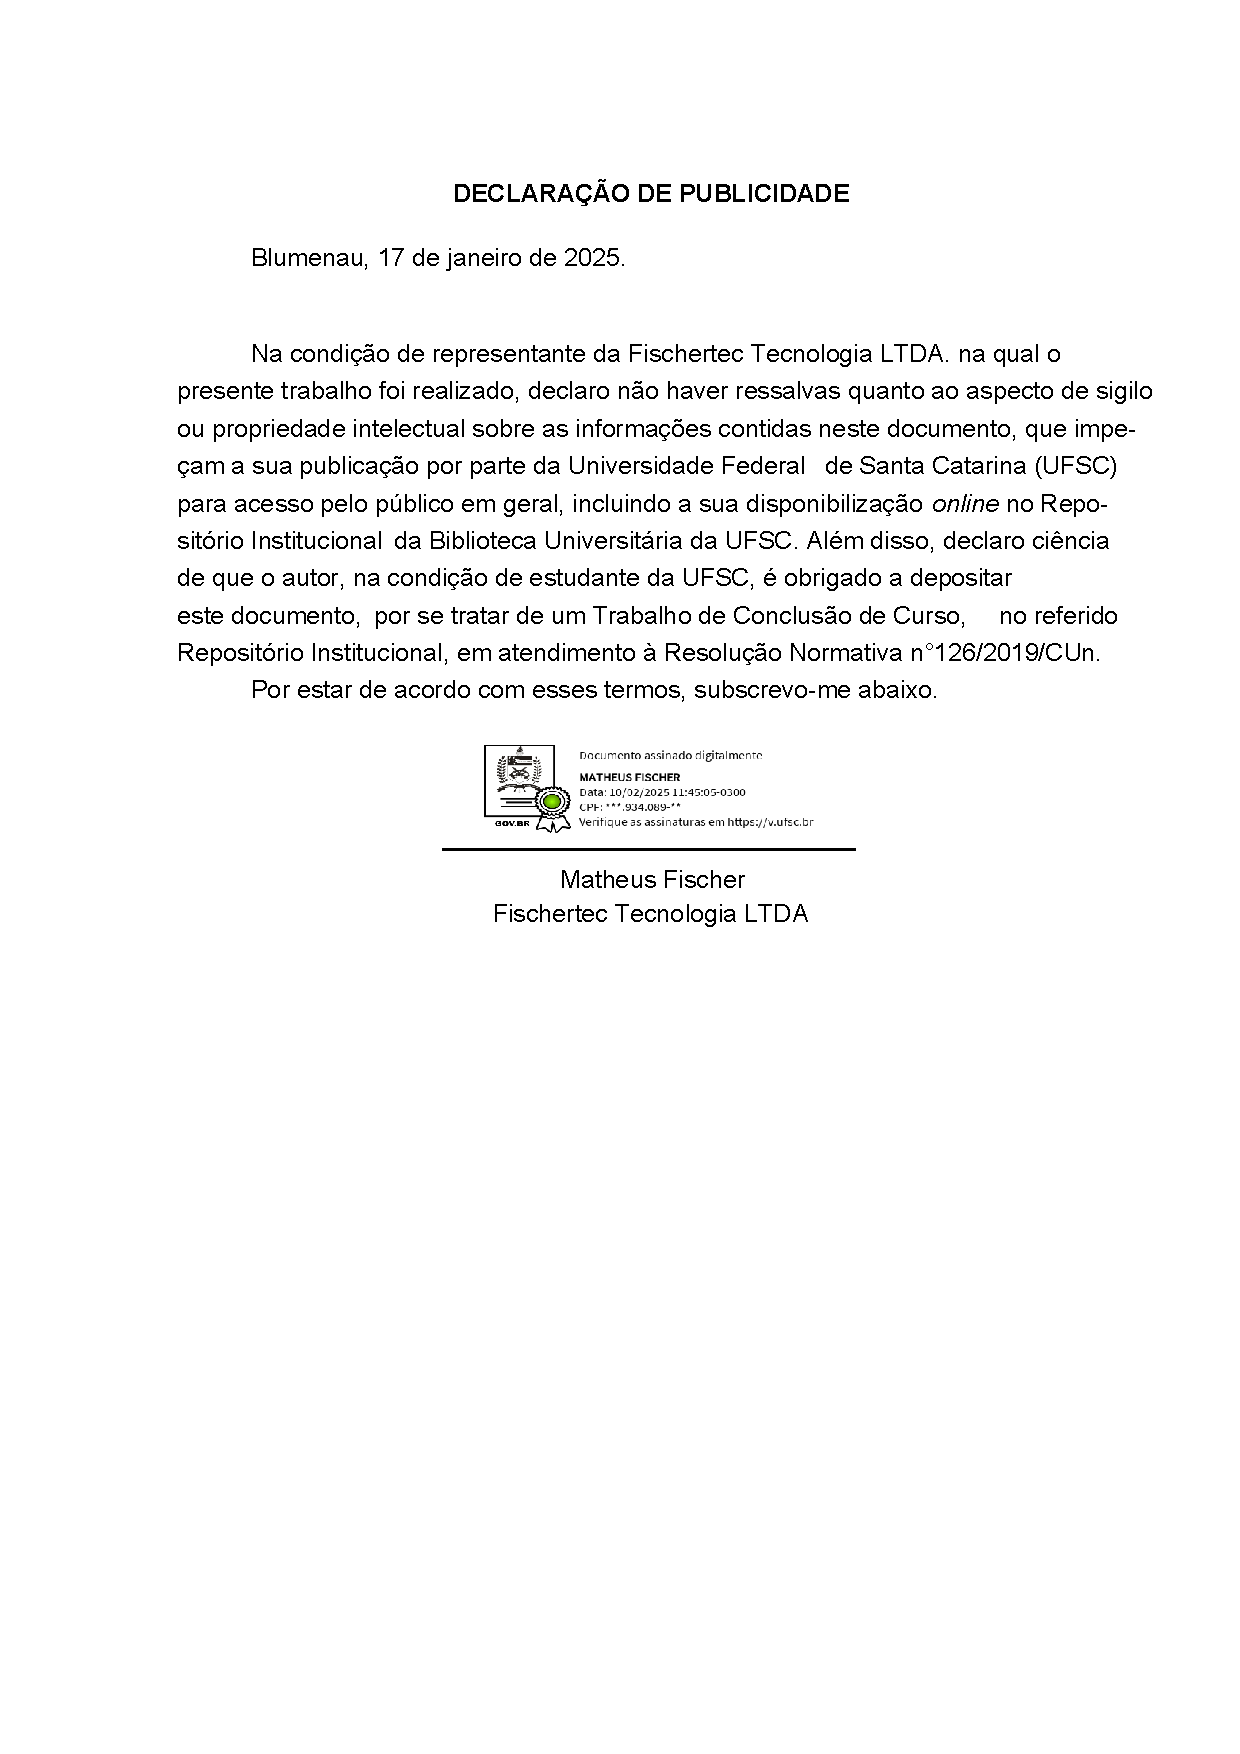
\includepdf{beforetext/Declaracao_publicidade_Fischertec_assinada.pdf}

% \begin{center}
% 	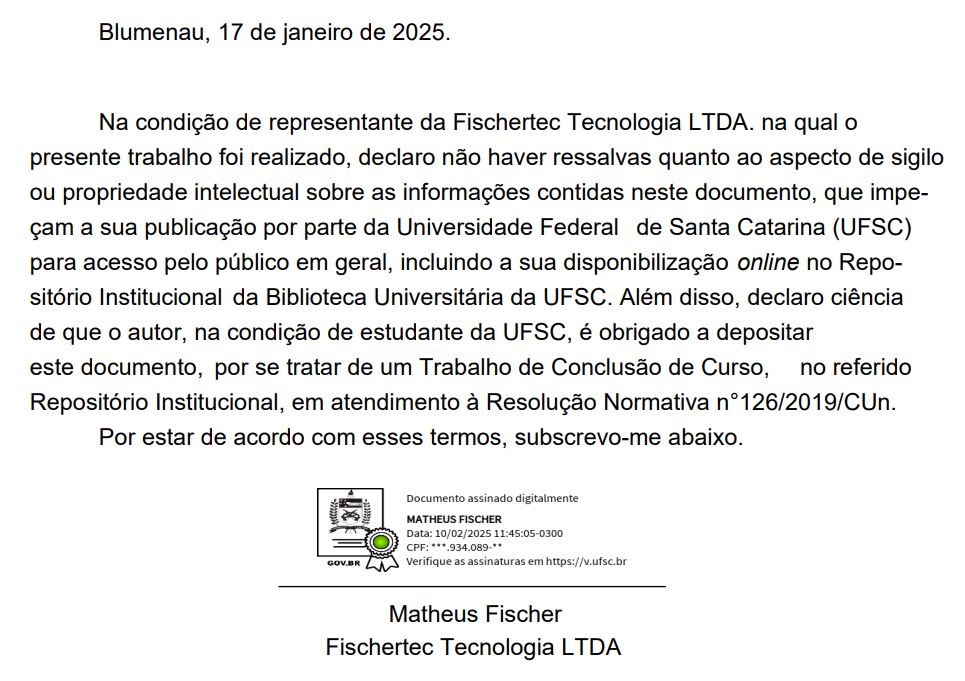
\includegraphics[scale=0.62]{beforetext/publicidade.png}
% \end{center}

% % Atenção: atualize o conteúdo de <texto>.

% % <Nome da cidade>, <dia> de <mês> de <ano>.
% Blumenau, 17 de janeiro de 2025.

% \vspace{1cm}

% Na condição de representante da <instituição de realização do PFC> na qual o presente trabalho foi realizado, declaro não haver ressalvas quanto ao aspecto de sigilo ou propriedade intelectual sobre as informações contidas neste documento, que impeçam a sua publicação por parte da Universidade Federal de Santa Catarina (UFSC) para acesso pelo público em geral, incluindo a sua disponibilização \emph{online} no Repositório Institucional da Biblioteca Universitária da UFSC. Além disso, declaro ciência de que o autor, na condição de estudante da UFSC, é obrigado a depositar este documento, por se tratar de um Trabalho de Conclusão de Curso, no referido Repositório Institucional, em atendimento à Resolução Normativa n° 126/2019/CUn.

% Por estar de acordo com esses termos, subscrevo-me abaixo.

% \vspace{15mm}

% \begin{center}
% 	\rule{7cm}{0.7pt} \\
% 	Matheus Fischer, Eng. \\
% 	Fischertec Tecnologia
% \end{center}

\cleardoublepage

% \includepdf{beforetext/Declaracao_publicidade_Fischertec_assinada2.pdf}

% \begin{fichacatalografica}
% 	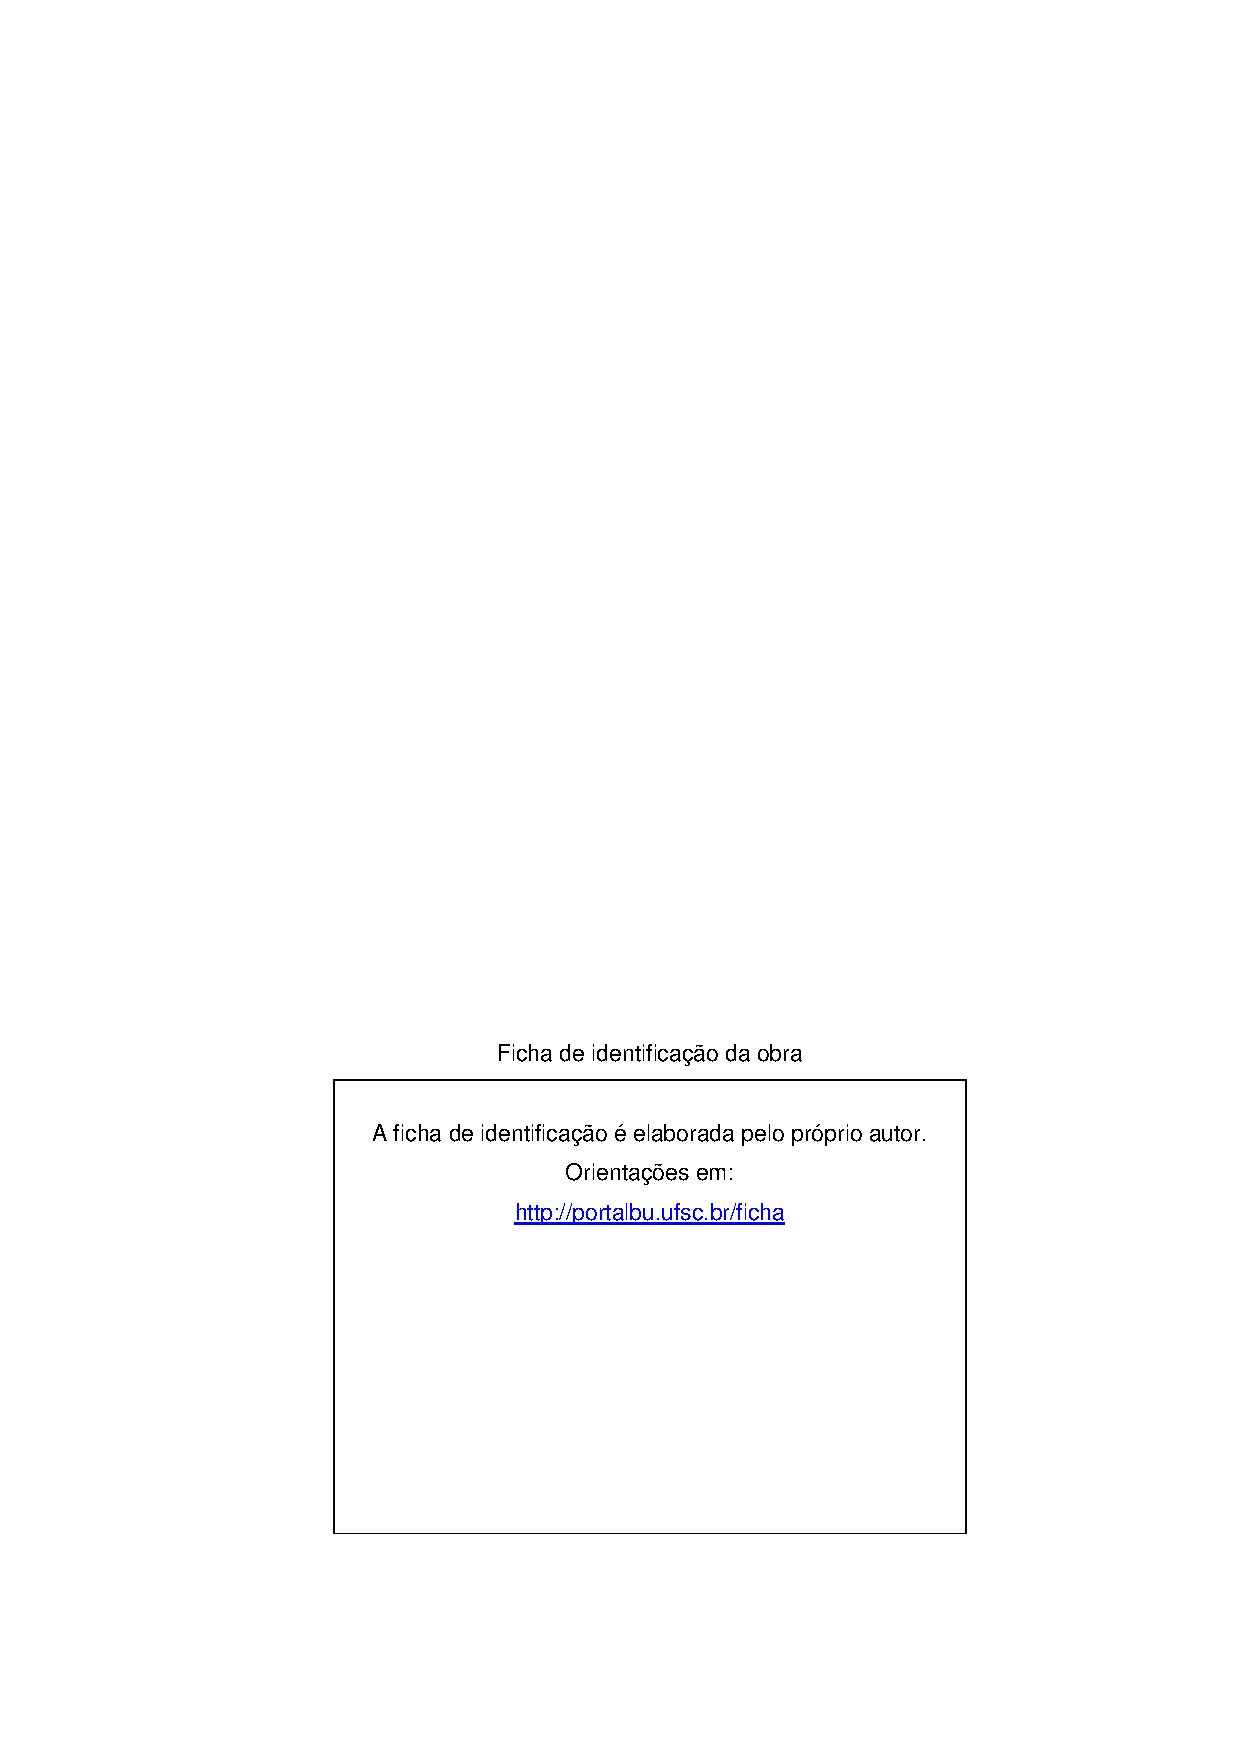
\includepdf{beforetext/Ficha_Catalografica.pdf}
% \end{fichacatalografica}

% ---
% RESUMOS
% ---

% resumo em português
% \setlength{\absparsep}{18pt} % ajusta o espaçamento dos parágrafos do resumo
% \begin{resumo}
% 	\SingleSpacing
% 	\textbf{Instruções do padrão genérico de TCCs da BU:}
% 	No Resumo são ressaltados o objetivo da pesquisa, o método utilizado, as discussões e os resultados com destaque apenas para os pontos principais. O resumo deve ser significativo, composto de uma sequência de frases concisas, afirmativas, e não de uma enumeração de tópicos. Não deve conter citações. Deve usar o verbo na voz ativa e na terceira pessoa do singular. O texto do resumo deve ser digitado, em um único bloco, sem espaço de parágrafo. O espaçamento entre linhas é simples e o tamanho da fonte é 12. Abaixo do resumo, informar as palavras-chave (palavras ou expressões significativas retiradas do texto) ou, termos retirados de thesaurus da área. Deve conter de 150 a 500 palavras. O resumo é elaborado de acordo com a NBR 6028. 
	
% 	\textbf{Instruções da Coordenação de PFC:} O Resumo deve descrever de forma sucinta: o contexto/motivação/problema tratado no PFC; a solução proposta; a implementação/desenvolvimento; a metodologia e as principais técnicas e ferramentas utilizadas; os principais resultados obtidos e a importância/impactos de tais resultados para a empresa/clientes da empresa/instituto de pesquisa. Escrever todos esses pontos de forma bem resumida e direta, e sem entrar em detalhes técnicos. O tamanho do Resumo deve ocupar praticamente esta página inteira, e num \textbf{único} parágrafo. Além disso, Resumo + Palavras-Chave não podem ultrapassar esta página. 
		
% 	\textbf{Palavras-chave}: Palavra-chave 1. Palavra-chave 2. Palavra-chave 3. \emph{[essas palavras-chave devem obrigatoriamente ser utilizadas no Resumo]}
% \end{resumo}
\setlength{\absparsep}{18pt} % ajusta o espaçamento dos parágrafos do resumo
\begin{resumo}
	\SingleSpacing
	A Fischertec Tecnologia é uma empresa brasileira que se concentra no desenvolvimento de soluções digitais de alta qualidade. Atua no setor de sites, aplicativos, e-commerces e diversos produtos digitais, buscando transformar ideias em soluções bem projetadas e inovadoras.

	O principal objetivo deste PFC é criar um \acrfull{MVP} de uma plataforma de agendamento de reservas de quadras esportivas em uma aplicação \acrfull{SaaS}. A criação desse sistema foi motivada pelas demandas específicas das empresas esportivas, como personalização de horários, preços e integrações com dispositivos \acrfull{IoT}.

	A Fischertec busca fornecer uma solução robusta, eficiente e alinhada às melhores práticas de automação e gestão esportiva. Ela optou por desenvolver um sistema proprietário que ofereça a experiência dos clientes empresariais com um produto único e personalizável, em busca da redução de sua dependência de projetos externos.

	O desenvolvimento da aplicação do servidor, que é o escopo deste PFC, utiliza Nest.js para a \acrshort{API} \acrshort{REST}, PostgreSQL como banco de dados e Docker para conteinerização. O sistema \textit{frontend}, em Next.js/React, será responsável pela interface do usuário em um futuro desenvolvimento. A metodologia utilizada foi ágil, garantindo entregas iterativas e validações frequentes com o TypeORM para persistência de dados. Postman serve como ferramenta de testes da \acrshort{API}.

	O principal resultado obtido é a entrega de uma aplicação \textit{backend} totalmente funcional que permite o gerenciamento completo de locações, com autenticação e controle de usuários e papéis para diferentes \textit{tenants} e preparada para uma futura integração com interface gráfica web. O sistema se mostrou eficiente, alinhado aos objetivos propostos e de fácil usabilidade.

	A aplicação do servidor é totalmente original e inovadora, destacando-se na resolução dos problemas enfrentados pela Fischertec ao simular um cenário real de operação.

	\textbf{Palavras-chave}: \acrshort{SaaS}. Nest.js. \acrshort{IoT}. Desenvolvimento. Software. \textit{backend}. Quadras. Esportivas. Gerenciamento. Agendamento
\end{resumo}

% % resumo em inglês
% \begin{resumo}[Abstract]
% 	\SingleSpacing
% 	\begin{otherlanguage*}{english}
% 		Resumo traduzido para outros idiomas, neste caso, inglês. Segue o formato do resumo feito na língua vernácula. As palavras-chave traduzidas, versão em língua estrangeira, são colocadas abaixo do texto precedidas pela expressão “Keywords”, separadas por ponto.
		
% 		\textbf{Keywords}: Keyword 1. Keyword 2. Keyword 3.
% 	\end{otherlanguage*}
% \end{resumo}

% resumo em inglês
\begin{resumo}[Abstract]
	\SingleSpacing
	\begin{otherlanguage*}{english}
		The Fischertec Tecnologia is a Brazilian company focused on providing high-quality digital solutions. It operates in the fields of websites, applications, e-commerce, and various digital products, with a focus on transforming ideas into well-designed and innovative solutions.

		The main objective of this PFC is to create a \acrfull{MVP} of a sports fields reservations management platform in a \acrfull{SaaS} environment. The creation of this system was motivated by the specific needs of sports industry companies, such as customizable schedules, prices, and IoT device integrations.

		The Fischertec company aims to provide a robust, efficient, and aligned with best practices solution for sports enthusiasts by offering an unique and personalized product experience. They opted to develop an owner-owned solution that aims to reduce their dependency on external projects.
		During this PFC project, the server application development scope is focused. It uses Nest.js for the \acrshort{REST} \acrshort{API}, PostgreSQL as the database, and Docker for containerization. The \textit{frontend} system in Next.js/React will be responsible for the graphical user interface in a future development.
		The methodology used was agile, ensuring iterative deliveries and frequent validations with TypeORM for data persistence. Postman is used as a tool for testing the \acrshort{API}.
		The main result obtained is the delivery of a fully functional backend application that allows comprehensive management and booking/scheduling of sports locations, with authentication and user roles for different tenants. The system was efficient and aligned with the proposed objectives and easy to use.

		The server-side application is original and innovative, standing out in the resolution of issues faced by the Fischertec company through simulating a real operation scenario.
		
		\textbf{Keywords}: \acrshort{SaaS}. Nest.js. \acrshort{IoT}. Development. Software. Backend. Fields. Sports. Management. Booking. Scheduling.
	\end{otherlanguage*}
\end{resumo}

%% resumo em francês 
%\begin{resumo}[Résumé]
% \begin{otherlanguage*}{french}
%    Il s'agit d'un résumé en français.
% 
%   \textbf{Mots-clés}: latex. abntex. publication de textes.
% \end{otherlanguage*}
%\end{resumo}
%
%% resumo em espanhol
%\begin{resumo}[Resumen]
% \begin{otherlanguage*}{spanish}
%   Este es el resumen en español.
%  
%   \textbf{Palabras clave}: latex. abntex. publicación de textos.
% \end{otherlanguage*}
%\end{resumo}
%% ---

{%hidelinks
	\hypersetup{hidelinks}
	% ---
	% inserir lista de ilustrações
	% ---
	\pdfbookmark[0]{\listfigurename}{lof}
	\listoffigures*
	\cleardoublepage
	% ---
	
	% ---
	% inserir lista de quadros
	% ---
	% \pdfbookmark[0]{\listofquadrosname}{loq}
	% \listofquadros*
	% \cleardoublepage
	% ---
	
	% ---
	% inserir lista de tabelas
	% ---
	\pdfbookmark[0]{\listtablename}{lot}
	\listoftables*
	\cleardoublepage
	% ---
	
	% ---
	% inserir lista de abreviaturas e siglas (devem ser declarados no preambulo)
	% ---
	\imprimirlistadesiglas
	% ---
	
	% ---
	% inserir lista de símbolos (devem ser declarados no preambulo)
	% ---
	% \imprimirlistadesimbolos
	% ---
	
	% ---
	% inserir o sumario
	% ---
	\pdfbookmark[0]{\contentsname}{toc}
	\tableofcontents*
	\cleardoublepage
	
}%hidelinks
% ---